\section{Evaluation}
\subsection{Experiments Setup}
\paragraph{Models and Baselines.}
We evaluate \cubic across three representative generative settings: text-to-image generation using Flux-1-dev~\cite{flux}, instruction-guided image editing using FireRed-Image-Edit-1.0~\cite{firered}, and text-to-video generation using Wan2.1-T2V-1.3B~\cite{wan}. We compare with state-of-the-art feature caching baselines, including TokenCache (ToCa)~\cite{tokencache}, TeaCache~\cite{teacache}, Pyramid Attention Broadcast (PAB)~\cite{pab}, and TaylorSeer~\cite{taylorseer}. 

\paragraph{Metrics and Evaluation Datasets} We measure acceleration using the end-to-end latency under the default inference settings of each task. Generation quality is evaluated with PSNR, SSIM, LPIPS, and FID/FVD for both image and video outputs. For image generation, we additionally report HPSv3~\cite{HPSv3}, while video generation is further evaluated using VBench metrics. Experiments are conducted on t2i-diversity-eval~\cite{brack2025howtotrain}, PIE-Bench++~\cite{Pie_bench}, and VBench~\cite{vbench} for image generation, image editing, and video generation, respectively.

\paragraph{Implementation} 
\label{sec:Implementation}
Experiments run on NVIDIA H100 using PyTorch. \cubic acts as a non-intrusive wrapper, with all methods sharing identical prompts and seeds for fair comparison. For caching baselines, we use their official implementations on Flux and Wan; for FireRed, which lacks official baseline support, we implement compatible versions (details in Appendix.~\ref{app:detail_result}). Our full codebase will be open-sourced.

\subsection{Main Results: Pareto-Optimal Acceleration}
\paragraph{Quantitative Comparison}
% 可以看到，Cubic在加速比更高的同时，比起其他cache加速方法达到了更高的生成质量。值得注意的是，对于attention在计算中耗时更大的模型（wan2.1),cubic更容易实现更高的加速。
We evaluate the quality and efficiency of images and videos generated with \cubic (std: $\rho=2$, fast: $\rho=4$) against baseline methods, and summarize the results in Table \ref{tab:results}. Compared with existing caching-based acceleration methods, \cubic achieves higher speedups while preserving better generation quality. Notably, for models where attention accounts for a larger fraction of the overall computation, such as Wan2.1, \cubic can remove redundant computation more effectively, leading to more pronounced acceleration gains.
\begin{table*}[t]
\centering
\caption{Quantitative evaluation of inference efficiency and visual quality in generation models.}
\resizebox{\textwidth}{!}{
\begin{tabular}{l c c c c c c c c}
\toprule
\textbf{Model} & \textbf{Method} 
& $\mathrm{Latency(s)}\downarrow$ 
& $\mathrm{Speedup}\uparrow$
& $\mathrm{PSNR}\uparrow$ 
& $\mathrm{SSIM}\uparrow$ 
& $\mathrm{LPIPS}\downarrow$ 
& $\mathrm{FID/FVD}\downarrow$ 
& $\mathrm{HPSv3/VBench}\uparrow$ \\
\midrule

\multirow{7}{*}{\textbf{Flux-1}} 
& $\mathrm{Baseline}$ & $11.59\pm0.05$ & -- & -- & -- & -- & -- & 10.68 \\
& $\mathrm{PAB}$ & $6.40\pm0.11$ & 1.81$\times$ & 20.37 & 0.7702 & 0.2574 & 77.37 & 10.65 \\
& $\mathrm{TeaCache}$ & $6.24\pm0.08$ & 1.86$\times$ & 22.88 & 0.8514 & 0.1490 & 45.87 & 10.83 \\
& $\mathrm{ToCa}$ &$ 6.39\pm0.04$ & 1.81$\times$ & 19.68 & 0.7493 & 0.2726 & 70.76 & 10.62 \\ 
& $\mathrm{TaylorSeer}$ & $6.83\pm0.08$ & 1.70$\times$ & 26.29 & 0.8920 & 0.0994 & \textbf{26.80} & 10.82 \\
\rowcolor{lightbluerow}
& \cubic~(std) & $6.14\pm0.24$ & 1.89$\times$ & \textbf{27.78} & \textbf{0.8998} & \textbf{0.0946} & 27.81 & 10.87 \\
\rowcolor{lightbluerow}
& \cubic~(fast) & $\mathbf{4.82\pm0.21}$ & \textbf{2.40$\times$} & 25.14 & 0.8457 & 0.1730 & 47.32 & \textbf{10.97} \\

\midrule

\multirow{7}{*}{\textbf{FireRed}} 
& $\mathrm{Baseline}$ & $39.14\pm0.09$ & -- & -- & -- & -- & -- & 8.17 \\
& $\mathrm{PAB}$ & $23.70\pm0.17$ & 1.65$\times$ & 24.39 & 0.8888 & 0.0929 & 39.41 & 7.95 \\
& $\mathrm{TeaCache}$ & $16.91\pm0.26$ & 2.31$\times$ & 23.80 & 0.8955 & 0.0995 & 41.03 & 7.83 \\
& $\mathrm{ToCa}$ & $20.06\pm0.04$ & 1.95$\times$ & 21.09 & 0.7884 & 0.1779 & 67.25 & 7.18 \\
& $\mathrm{TaylorSeer}$ & $21.04\pm0.04$ & 1.86$\times$ & 25.12 & 0.9102 & 0.0837 & 33.70 & \textbf{8.07} \\
\rowcolor{lightbluerow}
& \cubic~(std) & $18.26\pm0.57$ & 2.14$\times$ & \textbf{30.67} & \textbf{0.9538} & \textbf{0.0468} & \textbf{18.55} & 8.00 \\
\rowcolor{lightbluerow}
& \cubic~(fast) & $\mathbf{16.83\pm0.42}$ & \textbf{2.33$\times$} & 27.81 & 0.9201 & 0.0907 & 32.18 & 7.90 \\

\midrule

\multirow{7}{*}{\textbf{Wan 2.1}} 
& $\mathrm{Baseline}$ & $101.54\pm2.40$ & -- & -- & -- & -- & -- & 79.90 \\
& $\mathrm{PAB}$ & $40.60\pm0.10$ & 2.50$\times$ & 22.36 & 0.8000 & 0.1670 & 57.78 & 78.41 \\
& $\mathrm{TeaCache}$ & $61.44\pm1.92$ & 1.65$\times$ & 30.27 & 0.9270 & 0.0454 & 11.72 & 79.79 \\
& $\mathrm{ToCa}$ & $44.00\pm2.26$ & 2.31$\times$ & 19.19 & 0.7383 & 0.2405 & 84.04 & 78.42 \\
& $\mathrm{TaylorSeer}$ & $39.24\pm2.56$ & 2.59$\times$ & 15.80 & 0.6410 & 0.3521 & 137.06 & 78.82 \\
\rowcolor{lightbluerow}
& \cubic~(std) & $62.35\pm2.77$ & 1.63$\times$ & \textbf{32.76} & \textbf{0.9481} & \textbf{0.0317} & \textbf{7.92} & 79.37 \\
\rowcolor{lightbluerow}
& \cubic~(fast) & $\mathbf{37.32\pm0.62}$ & \textbf{2.72$\times$} & 26.39 & 0.8740 & 0.0986 & 31.76 & \textbf{80.03} \\

\bottomrule
\end{tabular}
}
\label{tab:results}
\end{table*}
\vspace{-7pt}
\paragraph{Sensitivity Test on Quality-Latency Trade-off}
Fig.~\ref{fig:tradeoff} reports the PSNR--speedup trade-off of \cubic and the compared baselines across different models. 
Across a wide range of speedup ratios, \cubic consistently attains higher PSNR (with correspondingly stronger SSIM, LPIPS, and FID/FVD; see Appendix~\ref{app:detail_result}), thereby lying on the Pareto frontier of the quality--latency trade-off.


% 这些实验都在flux上面做就好
\subsection{Validating Theoretical Foundations}
\vspace{-7pt}
\paragraph{Accuracy of Curvature Estimation}
\begin{figure}[t]
    \centering
    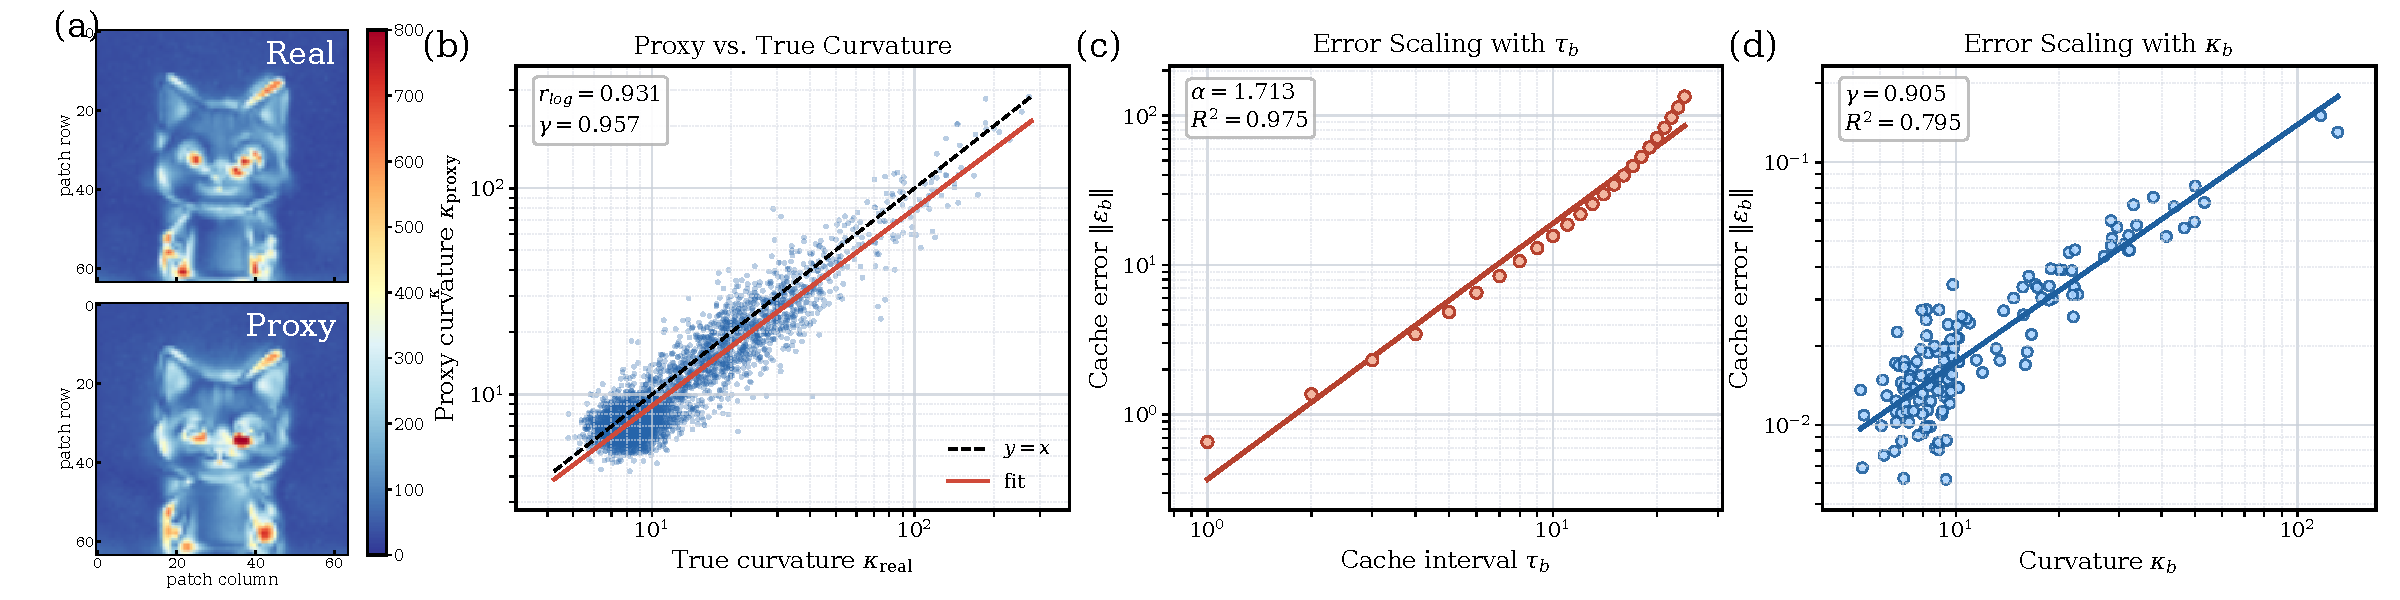
\includegraphics[width=\linewidth]{figure/theory.pdf}
    \caption{Validating the theoretical foundations of \cubic. (a) Visualization of real and proxy trajectory curvature on Flux. (b) Patch-wise correlation between $\kappa_{proxy}$ and $\kappa_{real}$. (c) Error scaling with reuse interval $\tau$. (d) Error scaling with curvature proxy $\kappa_b$.}
    \label{fig:theory_validation}
\end{figure}

We first validate whether the proposed endpoint-drift proxy accurately reflects true trajectory curvature. As shown in Fig.~\ref{fig:theory_validation}(a-b), the proxy closely matches both the spatial distribution and the relative magnitudes of the true curvature, exhibiting a strong linear correlation. This confirms that the proxy serves as a highly reliable online approximation for $\kappa^{(i)}$.

\vspace{-7pt}
\paragraph{Verification of the Cache Error Modeling}
We validate the cache-error bound derived in Eq.~\ref{eq:error_bound}. Fig.~\ref{fig:theory_validation}(c-d) confirm that the cache-induced error scales approximately quadratically with the reuse interval $\tau$ and linearly with the curvature proxy $\kappa$. These empirical scaling laws perfectly align with our theoretical derivations, demonstrating that the error model accurately captures the dominant behavior of cache-induced degradation.

% \paragraph{Optimality of Interval Allocation}
% % 相同speedup，验证-2/5次幂的tau分配生成效果是最好的。

\subsection{Ablation Studies on Core Components}

In Table.~\ref{tab:ablation}, we measure overhead and quality impact of \cubic components on Flux with standard setup.
\vspace{-7pt}
\paragraph{Monitor: Zero-Cost Proxy}
Despite introducing negligible system overhead, our drift proxy achieves generation quality remarkably close to that of the exact curvature computed via automatic differentiation. This validates our theoretical insight: the proxy successfully captures the essential trajectory geometry required for optimal scheduling, completely bypassing the prohibitive computational burden of explicit Jacobians.

\begin{wraptable}{r}{0.37\textwidth}
\vspace{-12pt}
\centering
\caption{Ablation Studies.}
\label{tab:ablation}
\footnotesize
\setlength{\tabcolsep}{3pt}
\renewcommand{\arraystretch}{0.95}
\begin{tabular}{@{}l c c c@{}}
\toprule
\textbf{Variant} & \textbf{Over.} & \textbf{FID}$\downarrow$ & \textbf{SSIM}$\uparrow$ \\
\midrule
\multicolumn{4}{l}{\footnotesize\itshape Monitor} \\
\quad Exact Jacobian & 603.9 & 33.1 & 0.967 \\
\rowcolor{lightbluerow}
\quad Proxy & \textbf{1.64} & 37.5 & 0.964 \\
\midrule
\multicolumn{4}{l}{\footnotesize\itshape Partitioner} \\
\quad Per-Token & 123.9 & 57.4 & 0.952 \\
\rowcolor{lightbluerow}
\quad Block-wise & \textbf{6.97} & \textbf{37.5} & \textbf{0.964} \\
\midrule
\multicolumn{4}{l}{\footnotesize\itshape Sparse Executor} \\
\quad w/o KV & 1.83 & 87.5 & 0.923 \\
\quad Static KV & 2.08 & 74.7 & 0.932 \\
\rowcolor{lightbluerow}
\quad Dynamic KV & 2.12 & \textbf{37.6} & \textbf{0.964} \\
\bottomrule
\end{tabular}
\vspace{-10pt}
\end{wraptable}


\vspace{-7pt}
\paragraph{Partitioner: Spatial Locality}
While per-token scheduling theoretically offers maximum flexibility, it incurs prohibitive indexing overhead. \cubic's block-wise strategy exploits the spatial locality inherent in DiT attention, drastically reducing scheduling complexity while maintaining contextual coherence, thereby achieving superior fidelity over the fine-grained baseline.
\vspace{-7pt}
\paragraph{Sparse Executor: Dynamic KV and Linear Scaling}
While a static KV cache prevents contextual isolation, it inevitably accumulates staleness errors. Our dynamic in-place update mechanism seamlessly resolves this by continuously refreshing the KV pool, minimizing staleness at negligible I/O cost.
Notably, layer-wise KV caches introduce memory requirements that scales with sequence length and layer count (e.g., 0.35GB for Flux vs. 17.68GB for Wan). To ensure deployability on memory-constrained hardware, we integrate asynchronous CPU offloading, which completely eliminates the GPU memory footprint of the cache at a marginal 5\% latency overhead.

\begin{wrapfigure}{r}{0.37\columnwidth}
\vspace{-10pt}
\centering
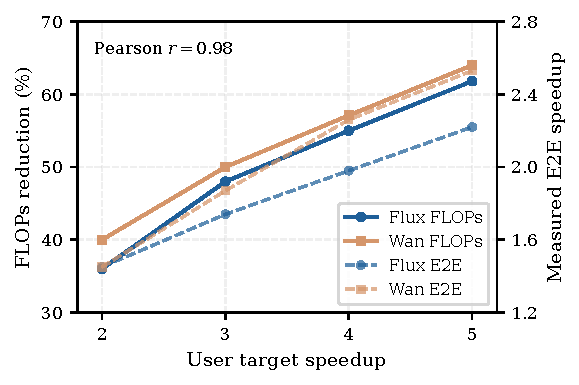
\includegraphics[width=\linewidth]{figure/flops.pdf}
\caption{FLOPs \& e2e speedup vs user-specified acceleration budget.}
\label{fig:flops}
\vspace{-10pt}
\end{wrapfigure}
Fig ~\ref{fig:flops} demonstrates that \cubic strategy effectively reduces flops in the selective phase, while the sparse executor efficiently transforms this into an end-to-end linear speedup. The speedup is lower than the user target because the speedup here only considers the selective phase; if end-to-end speedup is required, a simple conversion can be performed.



\subsection{Case Study: Components visualization}
\vspace{-7pt}
Due to space constraints, detailed visualizations of the dynamic pipeline are deferred to Appendix~\ref{app:case_study}. At a target speedup of $3\times$, \cubic executes five anchor steps. The scheduling exhibits a clear temporal evolution: early steps show high and heterogeneous curvature, leading to diverse interval allocations; middle steps capture localized high-curvature windows; and late steps converge to uniform curvature with consistent caching strategies. Throughout the process, the sparse ratio is stably maintained around $0.33$, and the step latency correlates strictly with the active ratio.